\chapter[Introduction]{Introduction}

\section{Motivation}

Humankind has only a few ways to generate reliable, nonintermittent 
base load power: fossil fuels, hydro-power, geothermal power, and 
nuclear energy. Because of increasing global warming and climate 
change concerns, sources with negligible CO$_2$ footprints 
are crucial measures for global temperature change control. 
From an environmental viewpoint, hydro and nuclear power are 
preferable ways to generate reliable power. Nevertheless, the 
potential for a hydro-power is strictly limited by local geographical 
conditions, hence, the only option left is nuclear power. Nuclear 
power plants generate 4.9\% of global energy \cite{noauthor_key_2017}. 
Moreover, a nuclear share in energy generation is projected to stay 
constant through 2040 while electricity demand will 
increase by 30\% \cite{noauthor_world_2017}. Unfortunately, a negative 
public attitude to nuclear was formed in many developed countries 
because of concerns regarding safety, nuclear weapons 
proliferation, radioactive waste treatment, and competitiveness with 
other sources of energy (i.e. renewables). This negative public 
attitude to nuclear energy makes it challenging to justify its zero 
emissions benefits.

Generation IV International Forum (GIF) chose \glspl{MSR} among the 
six advanced reactor concepts for further research and development. 
\glspl{MSR} 
offer significant improvements ``in the four broad areas of 
sustainability, economics, safety and reliability, and proliferation 
resistance and physical protection" \cite{doe_technology_2002}. To 
achieve the goals formulated by the GIF, \glspl{MSR} 
simplify the reactor core and improve inherent safety by using 
liquid coolant which is also a fuel\footnote{Herein \glspl{MSR} are 
assumed to be reactors with liquid fuel which simultaneously serves 
as coolant.}. In a thermal spectrum \gls{MSR}, liquid fuel is consists 
of carrier salt (i.e. LiF or LiF-BeF$_2$) and fluorides of fissile 
and/or fertile materials (i.e. UF$_4$, PuF$_3$ and/or ThF$_4$) 
which is circulates in a loop-type primary circuit 
\cite{haubenreich_experience_1970}. 
This innovation leads to immediate advantages over traditional, 
solid-fueled, reactors. These include near-atmospheric pressure 
in the primary loop, relatively high coolant temperature, outstanding 
neutron economy, a high level of inherent safety, reduced fuel 
preprocessing, the ability to continuously remove fission products 
and add fissile and/or fertile elements without shutdown 
\cite{leblanc_molten_2010}. The possibility of continuously removing 
neutron poisons increases the potential fuel burnup and thus 
improves the resource utilization of \glspl{MSR}. Finally, the \gls{MSR} 
also could be employed for transmutation of 
spent fuel from current \glspl{LWR} \cite{fratoni_design_2004}.

Recently, interest in \glspl{MSR} has resurged, with multiple new companies 
pursuing commercialization of \gls{MSR} designs\footnote{Examples 
include liquid-fueled molten salt designs from Terrapower, Terrestrial, 
ThorCon, Flibe, Copenhagen Atomics, etc.}. China's \gls{MSR} program 
was initiated in 2011 and promises to startup a 2MW$_{th}$ 
liquid-fueled test \gls{MSR} in 2020, a 10MW$_{th}$ 
demonstration reactor in 2025, and a gigawatt-level 
commercial reactor in 2050 \cite{zhang_review_2018}. The European 
Union funds the Safety Assessment of the Molten Salt Fast Reactor 
(SAMOFAR) project, in which several European research institutes and 
universities are developing various molten salt reactor prototypes 
such as the \gls{MSFR} \cite{fiorina_molten_2013} and the \gls{MOSART} 
\cite{ignatiev_molten_2014}.
To advance these \gls{MSR} concepts, particularly with respect 
to their strategies for online reprocessing and refueling, 
computational analysis methods capturing their unique reactor physics 
and process chemistry are needed.To correctly determine properties and 
operation of \glspl{MSR}, 
including injection/removal schemes, computational tools to accurately 
model the processes which are unique for this particular reactor type. 
Specifically, the circulation of the liquid fuel and the continuous 
feed or removal of elements (e.g. fissile material injection into 
and \glspl{FP} extraction from the fuel salt) are out-of-scope for 
most contemporary nuclear reactor physics software, which was  
originally written primarily to simulate solid-fueled reactors. 
Thus, a numerical simulation package able to model 
nuclear reactors with circulating fuel is needed to close the gap.

\section{Methodology}
The main objective of the proposed work is to develop the online 
reprocessing simulation package, SaltProc, which couples with 
the continuous-energy Monte Carlo depletion 
calculation code, SERPENT2 \cite{leppanen_serpent_2015}, 
for liquid-fueled \gls{MSR} simulations. The SaltProc package 
will enable the simulation of neutron poisons extraction 
based on mechanical and chemical models of fuel processing 
components. 
Moreover, it will take into account the non-instantaneous 
nature of injection/removal processes and material decay. 
The ultimate objective of this effort is to develop a generic 
open-source tool capable of simulating a wide range of 
liquid-fueled systems including two-fluid, multi-region 
designs, and validate it against existing modeling efforts. 
Figure~\ref{fig:workflow_method} illustrates 
the proposed plan towards the ultimate objective 
including my previous research effort towards and after 
master's degree.
\begin{figure}[htp!] % replace 't' with 'b' to 
  \centering
	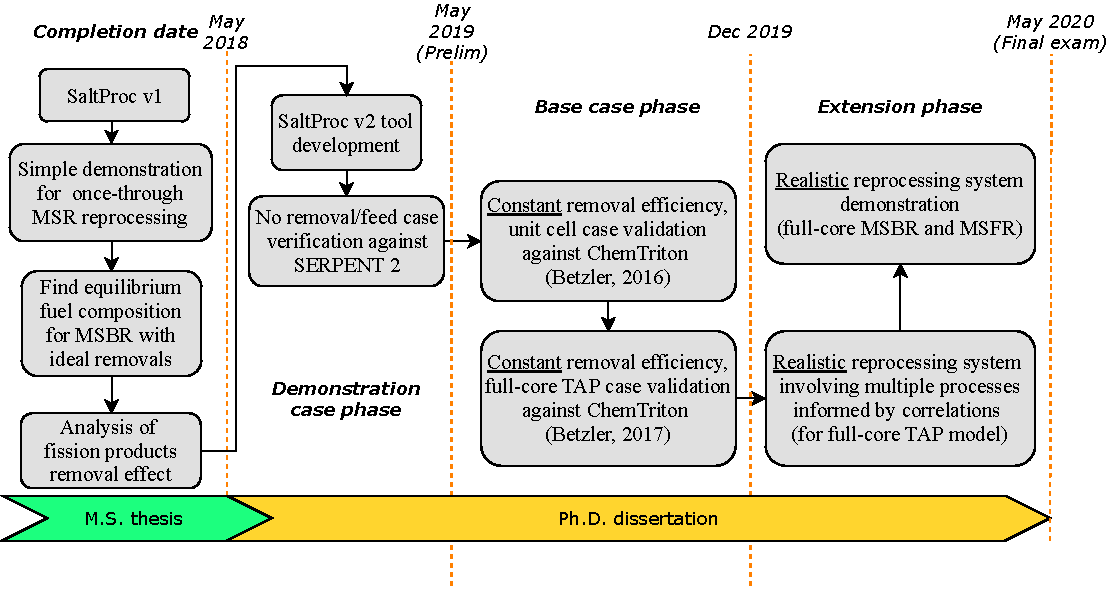
\includegraphics[width=\textwidth]{workflow_for_methodology.pdf}
  \caption{Workflow for completed (M.Sc. thesis) and proposed (Ph.D.) work 
  which includes the tool demonstration and validation for the \gls{TAP} 
  reactor, the \gls{MSBR}, and the \gls{MSFR}.}
  \label{fig:workflow_method}
\end{figure}

In Chapter 2 of this work, current published online reprocessing 
simulation efforts have been systematized, investigated and 
reviewed to identify desirable generic reprocessing tool capabilities. 
A preliminary set of key input 
and output parameters, software package architecture, and class 
structure are defined in Chapter 3 to realistically model a generic  
online reprocessing system. 

In Chapter 4, the proposed simulation package will be demonstrated and 
verified for three perspectives liquid-fueled \gls{MSR} with different 
key characteristics: fuel salt composition, number of salts (single- 
and two-fluid), neutron spectra, and reprocessing schemes. Specifically, 
these demonstration and verification efforts will focus on the \gls{TAP} 
\gls{MSR} because it well analyzed in the literature. 
SaltProc results will be verified against recent online reprocessing 
efforts in the literature for the \gls{TAP} reactor, the \gls{MSBR}, 
and the \gls{MSFR}. 

Chapter 5 will summarize the conclusions reached concerning the 
appropriate mechanical and chemical models of fuel processing 
components to utilize in the online reprocessing plant simulation. 
Moreover, phases of the proposed work will be described in detail. 
Finally, remaining future work and expected contributions to the 
nuclear community will be summarized.